% header stuff
% ------------

\documentclass[twocolumn, final]{svjour3}
\usepackage[square,numbers]{natbib}
\usepackage{amsmath, epsfig}
\usepackage{amsfonts}
\usepackage{graphicx}
\usepackage{amsfonts}
\usepackage{algorithm}
\usepackage{algorithmic}
\usepackage{easybmat}
\usepackage{footmisc}
\usepackage[usenames,dvipsnames]{color}
\usepackage{subfig}
\renewcommand\algorithmiccomment[1]{// \textit{#1}}
\newcommand{\ignore}[1]{}
\newcommand{\comment}[1]{}
\newcommand{\frank}[1]{\textcolor{red}{\textsf{\emph{\textbf{\textcolor{blue}{#1}}}}}}
\newcommand{\willie}[1]{\textcolor{green}{\textsf{\emph{\textbf{\textcolor{green}{#1}}}}}}
\DeclareMathOperator*{\argmax}{arg\,max}

\begin{document}


% title and author related
% ------------------------

\title{Unsupervised Detection and Tracking of Arbitrary Objects with Dependent Dirichlet Process Mixtures}
\titlerunning{Unsupervised Detection and Tracking of Arbitrary Objects with Dependent Dirichlet Process Mixtures}
\author{Willie Neiswanger$^{*}$ and Frank Wood$^{\dagger}$}
\authorrunning{Willie Neiswanger and Frank Wood}
\institute{ $^{*}$Columbia University, Department of Applied Math and Applied Physics. Tel.: 503-464-6152. \email{wdn2101@columbia.edu} \and $^{\dagger}$Columbia University, Department of Statistics. Tel.: 212-851-2150. \email{fwood@stat.columbia.edu}}
\date{}  % add submit date when submitted
\maketitle


% Abstract
% --------

\begin{abstract}
This paper proposes a technique for the unsupervised detection and tracking of arbitrary objects in videos. It is intended to reduce the need for detection or localization methods tailored to specific object types and serve as a general framework applicable to videos with varied objects, backgrounds, and film qualities. The technique uses a dependent Dirichlet process mixture (DDPM) known as the Generalized Polya Urn (GPUDDPM) to model image pixel data that can be extracted in a general manner from the regions in a video that represent objects. This paper describes a specific implementation of the model using spatial and color pixel data extracted via frame differencing and gives two algorithms for performing inference on the model to accomplish detection and tracking. This technique is demonstrated on multiple synthetic and benchmark video datasets that illustrate its ability to, without modification, detect and track objects with diverse physical charactersitics moving over non-uniform backgrounds and through occlusion.
% \keywords{Object Detection \and Tracking \and Bayesian Nonparametrics \and Multiple Target Tracking}
\end{abstract}



% introduction
% ------------

\section{Introduction}
\label{sec:introduction}

We define the task of automated detection and tracking of arbitrary objects in videos to be: extraction, localization, and tracking. Extraction is the task of determining the spatiotemporal regions of a video that constitute objects, localization is the task of finding the positions and/or shapes of distinct objects, and tracking is the task of maintaining the identities of the detected objects over time. An ability to carry out these tasks in an automated manner is useful for many fields that make use of video data, including robotics, video surveillance, time-lapse microscopy, and video summarization. Algorithms able to be applied to a variety of objects and video types are particularly desirable. This paper introduces a new framework involving the use of dependent Dirichlet process mixture models. This framework provides a foundation for a class of unsupervised algorithms that can detect and track arbitrary objects in a wide range of videos.

Research on methods for general detection and tracking of objects has focused on one of either extraction, localization, or tracking. Integrating all three tasks in a system for multiple arbitrary objects and diverse video types was not often a primary focus. Accomplishing the three tasks in a cohesive manner has been pursued more recently and has produced algorithms that can, in a fully automated way, accomplish unsupervised detection and tracking---or in short, that can determine the spatiotemporal region of a video occupied by distinct objects. An example of general detection and tracking is called ``blob tracking'', which typically refers to methods that perform extraction and localization of objects in each frame independently. Tracking involves finding blobs with similar locations and appearances over time. The main blob tracking challenges are the difficulty of segmenting neighboring or occluding objects in a given frame \cite{zhao2004tracking} and preventing multiple tracked blobs from merging into a single object \cite{vermaak_2003}. These difficulties stem from performing detection via segmentation on individual frames.

This paper presents the use of a Bayesian nonparametric mixture model for general, unsupervised multiple object detection and tracking. This method provides both a widely applicable way to detect arbitrary objects in videos---particularly in cases where frame-by-frame segmentation is difficult or video quality is low and extraction is noisy---and a general framework for identifying and isolating objects during tracking. Specifically, this work describes how a dependent Dirichlet process mixture model can accomplish these goals. The DDP is first reviewed in the abstract. This model can be used with arbitrary extraction procedures and object appearance representations that may be desired in future studies. We then present our specific model for data obtained via a basic extraction procedure. We describe inference algorithms for the DDP, and specifically our specific model, that allow object localization and tracking to be carried out. We demonstrate our implementation on multiple synthetic and benchmark datasets. Standard performance metrics for each supports our hypothesis that general extraction combined withe sophisticated inference can perform detection and tracking at a level comperable to state-of-the-art, object specific algorithms.



% Prior Work
% ----------

\section{Prior Work}
\label{sec:priorwork}

Many methods in the fields of image processing, signal processing, and computer vision have been developed to solve aspects of the problem of unsupervised detection and tracking of arbitrary objects. These methods might be placed into a few broad categories: those that aim to distinguish the foreground regions of images from the background, segment images into distinct regions, localize specified objects or features in images, track an object over a sequence of images (after its position has been specified in an initial image), track multiple objects over a sequence of images (especially when the objects interact or occlude one another), segment a sequence of images into distinct spatiotemporal regions, and combine the previous methods in some way to create systems capable of both detecting and tracking specified objects, or of discerning which regions of a video constitute distinct, arbitrary objects and tracking these.



% Overview
% --------

\section{Overview of Method}
\label{sec:overviewofmethod}

Successful methods for detecting and tracking objects in videos are often tailored for specific object types. These methods rely on ad-hoc detection criteria that exploit previous knowledge about the appearance or behavior of objects in a video. The method described in this paper is designed to track arbitrary objects without using any explicit detection criteria, and serve as a general strategy that can be used, without modification, to perform accurate detection and tracking of diverse objects in a wide range of videos. This method begins by performing a data extraction procedure (a consistent procedure for all videos), which can be carried out broadly but yields noisy data; we model this noisy extracted data with a sophisticated type of Bayesian mixture model. Inference can then be performed on this model to gain detection and tracking results.

This paper describes the data extraction procedures (Section~\ref{sec:dataextraction}), the general form of the model (Section~\ref{sec:modeloverview}), the specific distributions used in our implementation of the model (Section~\ref{sec:modelspecification}), and inference procedures used to get tracking results (Section~\ref{sec:inference}).



% Frame Diff and Longimg figure
% -----------------------------

\begin{figure*}
  \centering
  \subfloat[]{\label{fig:ants_img}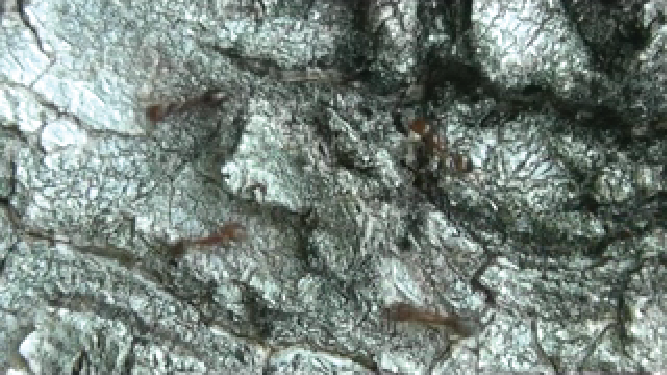
\includegraphics[width=0.335\textwidth]{../img/usbh_frame_723.pdf}} 
  \subfloat[]{\label{fig:ants_img2}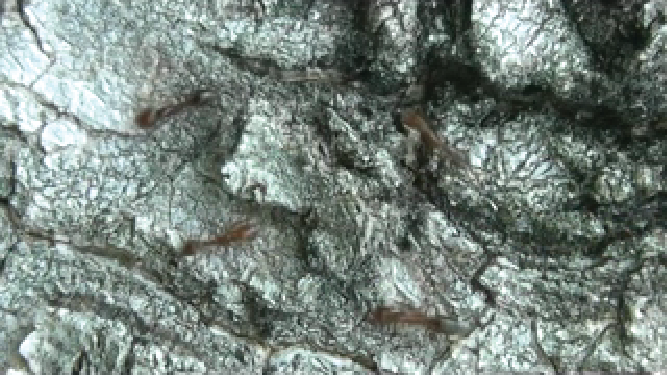
\includegraphics[width=0.335\textwidth]{../img/usbh_frame_724.pdf}}
  \subfloat[]{\label{fig:ants_img_framediff}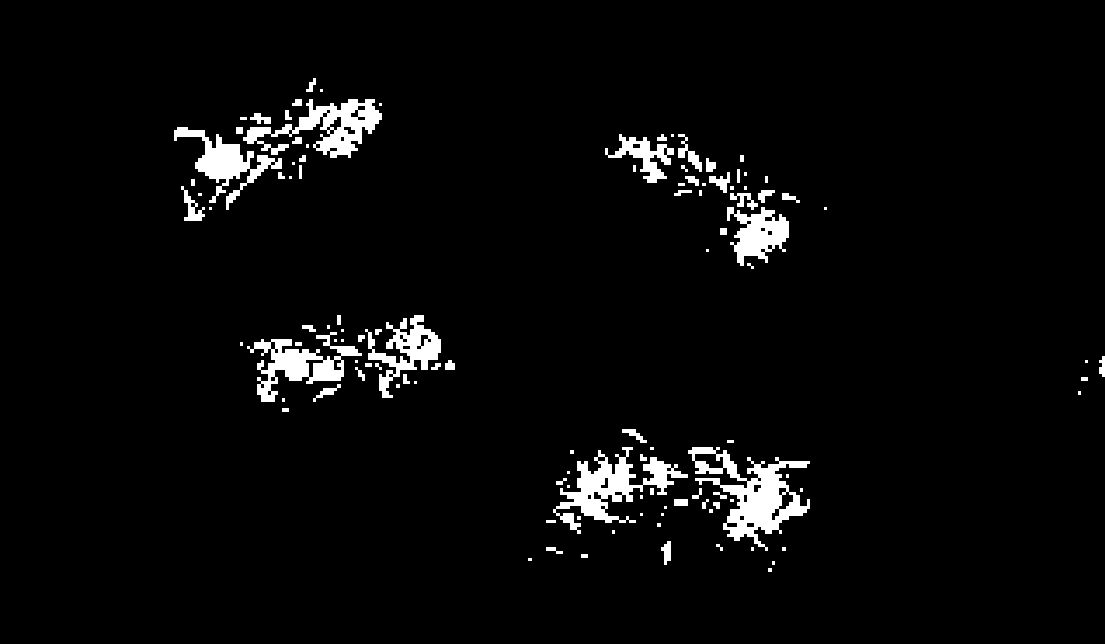
\includegraphics[width=0.323\textwidth]{../img/usbh_framediff.png}}\\
  \subfloat[]{\label{fig:traffic2_img}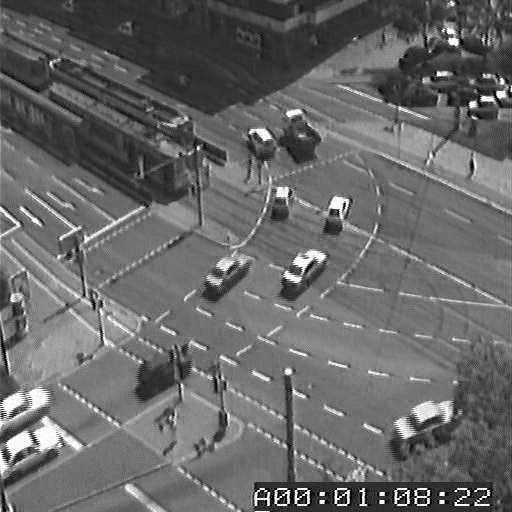
\includegraphics[width=0.328\textwidth]{../img/traffic2_frame1.png}} 
  \subfloat[]{\label{fig:traffic2_img2}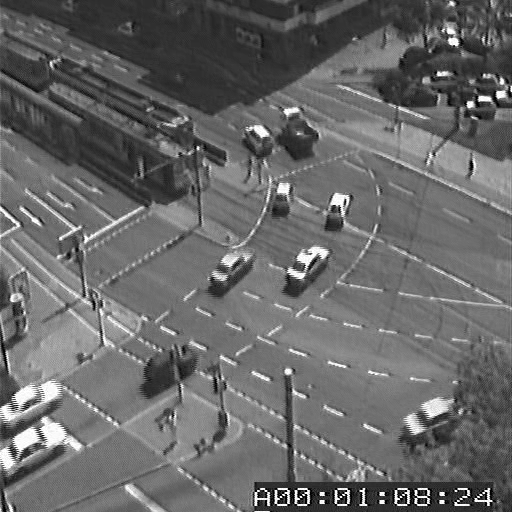
\includegraphics[width=0.328\textwidth]{../img/traffic2_frame2.png}}
  \subfloat[]{\label{fig:traffic2_img_framediff}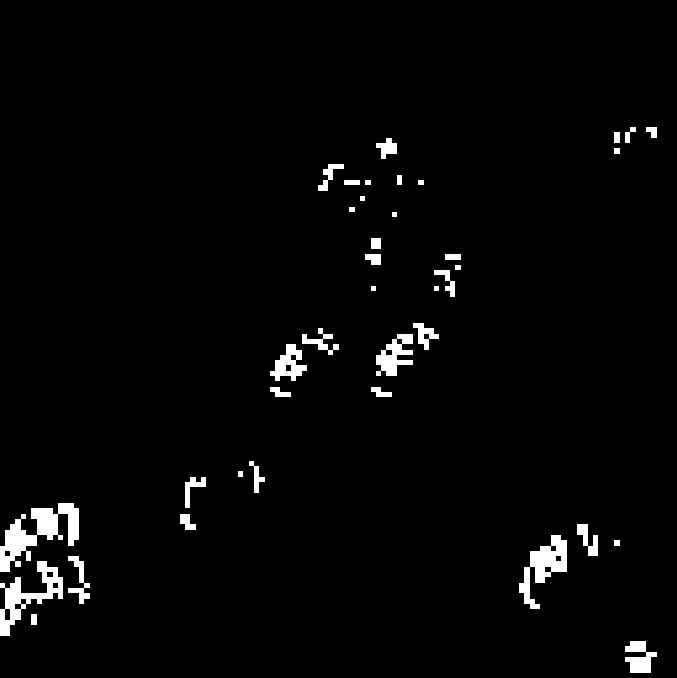
\includegraphics[width=0.3273\textwidth]{../img/traffic2_framediff.png}}\\
  \subfloat[]{\label{fig:pets2009_img}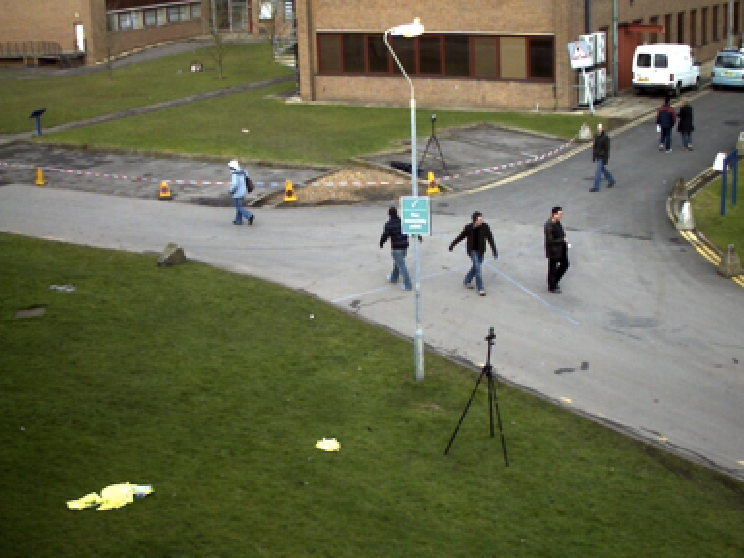
\includegraphics[width=0.333\textwidth]{../img/pets2009_frame1.png}} 
  \subfloat[]{\label{fig:pets2009_img2}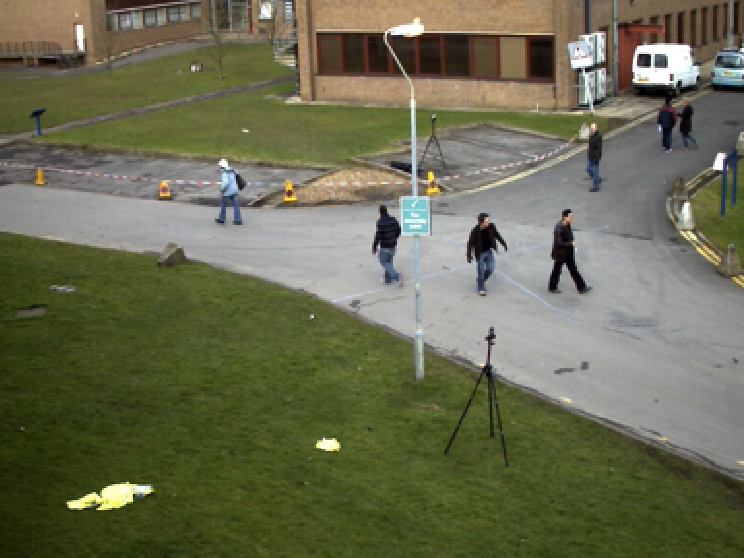
\includegraphics[width=0.333\textwidth]{../img/pets2009_frame2.png}}
  \subfloat[]{\label{fig:pets2009_img_framediff}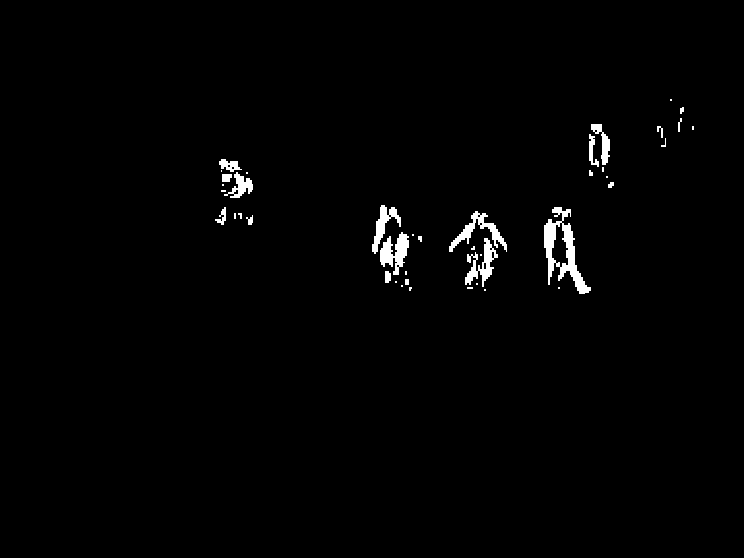
\includegraphics[width=0.333\textwidth]{../img/pets2009_framediff.png}}\\
  %\subfloat[]{\label{fig:longimg}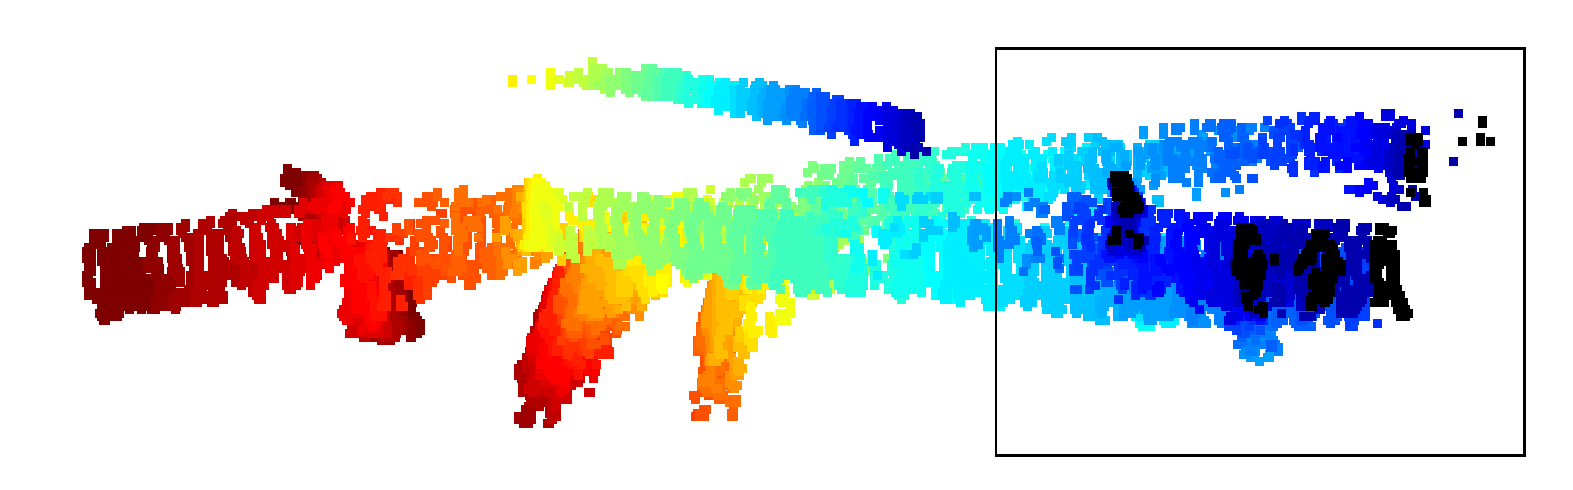
\includegraphics[width=1.05\textwidth]{../img/longimg_6.pdf}} \\
  \subfloat[]{\label{fig:longimg_all}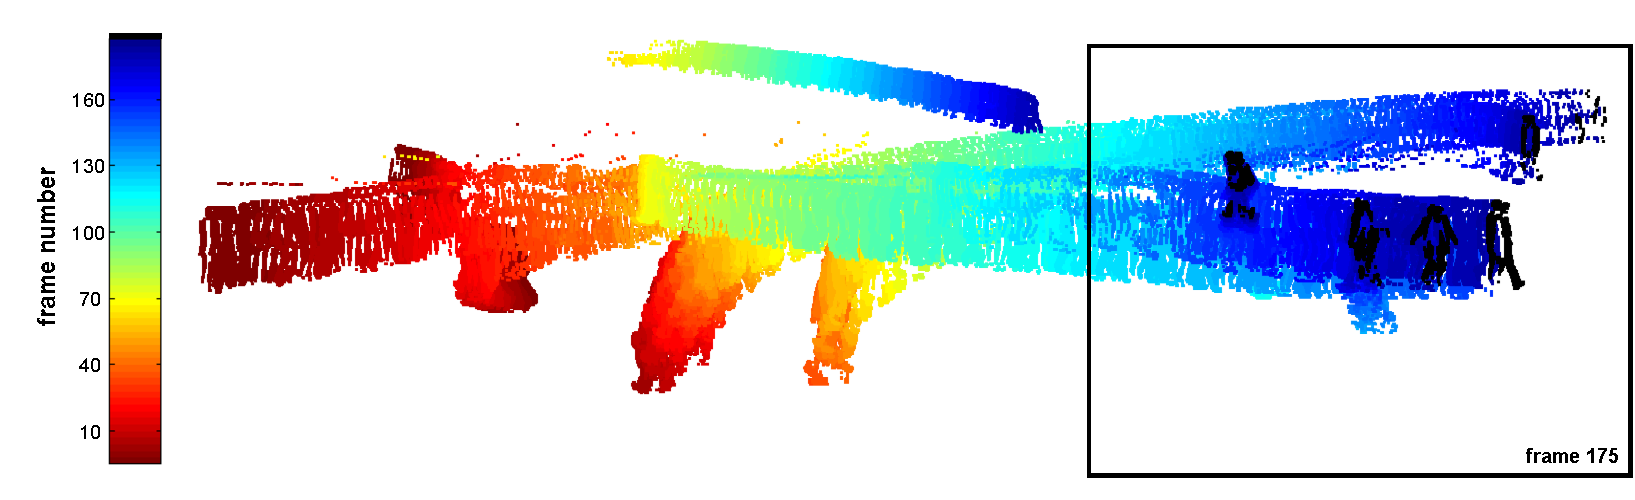
\includegraphics[width=1\textwidth]{../img/longimg_7_detail.pdf}} 
  \caption{Pairs of consecutive frames and the results produced by taking the pixel-wise difference between these frames (a - f). The final image shows the result of frame differencing over a sequence of images (from the PETS2009 dataset), where color denotes frame number.}
  \label{fig:img_and_framediff}
\end{figure*}



% Data Extraction
% ---------------

\section{Data Extraction}
\label{sec:dataextraction}

% General intuition/definition, possible extraction methods, example with frame differencing (cite figure).
% \\previous 3 data sections:
% \\a. general def, baseline data, other examples, idea that we are clustering to get results
% \\b. frame differencing def (+ color counting)
% \\c. specific form of data (specified frame diff params) used in experiments
% \\\\new plan: general intuition, baseline data, general def, (idea that we are clustering?), list of extraction examples, frame differencing def, color counting def\\


We defined the task of extraction to be the unsupervised determination of which spatiotemporal regions of a video constitute objects, and outlined a number of extraction methods in Section~\ref{sec:priorwork}. The most basic dataset that can be gained from extraction is comprised of the three-dimensional points $\bold{x} = ( x_{1}, x_{2}, t ) \in \mathbb{R}^{2} \times \mathbb{Z}_{+}$, where $x_{1}$ and $x_{2}$ are the two spatial dimensions of a pixel contained in a region found during extraction and $t$ is the frame in which the pixel resides. Once this dataset, which we will refer to as a ``baseline extraction dataset'', has been found, additional features may also be extracted from the video. Examples of additional features include color information, pixel intensity values, feature point (such as corner, shape, or edge) locations or spatial characteristics, and texture representations; the main idea is to choose features which are able to be easily extracted or computed, capture variability in the appearance of objects, and are applicable to a wide variety of object types.

The baseline extraction dataset has the appearance of worm-like clusters that follow the paths of individual objects as they move (as illustrated in Figure~\ref{fig:longimg_all}). Modeling this data with a dependent Dirichlet process mixture model (Section~\ref{sec:gpuddpmixture}) allows us to perform inference (Section~\ref{sec:inference}), which carries out clustering of the data. By choosing this type of model, we aim to provide a clustering result that isolates each worm-like cluster and infers a sequence of distributions for each, which we use to gain localization and tracking results for each object (Section~\ref{sec:inferencetotrackingresults}).

For implementation in experiments (Section~\ref{sec:experiments}), we desire an extraction procedure that is as unsophisticated as possible, both to gauge the robustness of this method on potentially noisy extraction data and to ensure that the procedure is applicable to a wide range of videos. Consequently, in all experiments we carry out a method called ``frame-differencing'', which locates motion by recording the positions of pixels that have exhibited differences in intensity or value in succesive frames beyond a given threshold. Frame differencing is unsophisticated, computationally inexpensive, able to be applied to a wide range of static, single-camera videos (note that videos used in all experiments were stationary; moving-camera videos require extraction methods that provide accurate foreground segmentation for non-stationary video). We have found that, when correctly implemented, frame differencing is sufficiently general to extract the desired worm-like clusters from a variety of videos containing multiple moving objects. A few examples of this extraction procedure on pairs of consecutive video frames can be found in Figure~\ref{fig:img_and_framediff}(a-i).

We furthermore wish to capture the color (or grayscale) value of each pixel and incorporate this color information into our model. For each pixel $x = (i, j, t)$ recorded during frame differencing, we specify a square, $L$ pixels in length, centered on $(i, j)$, that selects a set of pixels surrounding $\bold{x}$ in frame $t$. We also specify a scalar color value that is able to be computed for each pixel; this value could, for example, be some function of the red-green-blue (r-g-b) or hue-saturation-value (h-s-v) characteristic of a pixel. The color value of each of the selected pixels surrounding $\bold{x}$ is recorded. Afterwards, the set of possible color values (ie the range of color values to which a pixel may be assigned) is partitioned into $V$ bins, and the number of pixels with a color value lying in each of the bins yields a $V$ dimensional vector of `color counts'. We will refer to this extraction technique as `color counting'.

The frame differencing and color counting extraction yields a set of data $\bold{X} \subset \mathbb{R}^{2} \times \mathbb{Z}_{+}^{V} \times \{1, \ldots, T \}$, where each element $\bold{x} \in \bold{X}$ can be written
\begin{equation}
\bold{x} = ( \bold{x}^{s}, \bold{x}^{c}, t ) = ( x^{s_{1}}, x^{s_{2}}, x^{c_{1}}, \ldots, x^{c_{V}}, t )
\end{equation}
where $\bold{x}^{s} \in \mathbb{R}^{2}$ is the two dimensional vector of spatial coordinates,  $\bold{x}^{c} \in \mathbb{Z}_{+}^{V}$ is the $V$ discrete dimensional vector of color counts, and $t \in \{1, \ldots, T \}$ is the discrete time index. 

In the experiments described in Section~\ref{sec:experiments}, the hue component of the h-s-v value is recorded from all pixels that surround each extracted pixel $\bold{x}$ in the manner described above, choosing $L=5$. Additionally, the set of possible hue values is partitioned into 10 bins, and the number of pixels with a hue value lying in each of the 10 bins is recorded to yield the vector of ``color counts'' $\bold{x}^{c} = x^{c_{1}}, \ldots, x^{c_{10}}$. Hue is chosen to represent object color since it has been demonstrated in previous work as a simple representation of object appearance that allows for distinct objects to be well differentiated \cite{perez_2002, raja_1998, mckenna_1999}.



% Model Overview
% --------------

\section{Model Overview and General Form}
\label{sec:modeloverview}

Dirichlet Process Mixture (DPM) models (Section~\ref{sec:dpmixture}) fall under the heading of Bayesian nonparametric (BNP) models. These models have been widely used in the past decade to perform nonparametric density estimation and cluster analysis. Since we have time series data and wish to find spatiotemporal clusters, we are interested in using a closely related class of models known as Dependent Dirichlet Process Mixture (DDPM) models (Section~\ref{sec:ddpmixture}). These models are particularly useful for estimating the number of latent classes (clusters) in time dependent data. In this work, estimating the number of clusters in video extraction data is equivalent to estimating the number of distinct objects in a video.

This section provides background information that allows us to introduce DDPM models, describes the motivation behind our use of these models, and gives a definition of the particular DDPM chosen, known as the Generalized Polya Urn Dependent Dirichlet Process Mixture (GPUDDPM) model (Section~\ref{sec:gpuddpmixture}).


\subsection{Finite Mixture Model}
\label{sec:finitemixture}

A finite mixture model can be thought of as a probability distribution for an observation $x_{i}$ formulated as a linear combination of K mixture components (which we also refer to as `clusters'), where each mixture component is a probability distribution for $x_{i}$ with some parametric form, and the coefficients of the linear combination sum to one. The finite mixture model can be written as
\begin{equation}
P(x_{i}) = \sum_{k=1}^{K} P(c_{i} = k)P(x_{i}|\theta_{k})
\end{equation}
$\forall i \in \{ 1, \ldots, N \}$, where $c_{i} \in \{ 1, \ldots, K \}$ denotes the assignment of $x_{i}$ to a given mixture and $\theta_{k}$ denotes the parameters of the $k^{\text{th}}$ mixture component. Note that by choosing $P(c_{i} = k)$ as coefficients of the linear combination, it is ensured that these coefficients sum to one. We also define $p_{k} := P(c_{i} = k)$ for $k \in \{ 1, \ldots, K \} $. We can therefore write this model generatively as
\begin{align}
\begin{split}
	c_{i}|p_{1}, \ldots, p_{K}  &\sim  \text{Discrete}(p_{1}, \ldots, p_{K}) \\
	x_{i}|c_{i}, \theta_{c_{i}}  &\sim  \text{F}(\theta_{c_{i}})
\end{split}
\end{align}
$\forall i \in \{ 1, \ldots, N \}$, where the $x_{i}$ are observations, the $c_{i}$ are the mixture component assignments associated with each observation, the $\theta_{c_{i}}$ are parameters defining the $c_{i}^{\text{th}}$ mixture component (i.e. the distribution to be mixed, $\text{F}(\theta_{c_{i}})$), and the ``Discrete'' distribution refers to a multinomial distribution whose parameters are a 1-of-K vector (i.e. a vector of counts that sums to one).


\subsection{Bayesian (Finite) Mixture Model}
\label{sec:bayesianmixture}

The finite mixture model of Section~\ref{sec:finitemixture} can be extended to a Bayesian mixture model by viewing parameters that were previously point values, $\theta_{c_{i}}$ (the mixture component parameters) and $p_{1}, \ldots, p_{K}$ (the mixture component assignment weights), as random variables and providing each with a prior distribution. In this case, the prior distribution $\mathbb{G}_{0}$ is placed on the mixture component parameters, and the prior distribution $\text{Dir}(\alpha/K, \ldots, \alpha/K)$ is placed on the mixture component assignment weights. The resulting Bayesian mixture model can be formulated generatively as
\begin{align}
\begin{split}
\label{bayesian_mixture_model}
	p_{1}, \ldots, p_{K}  &\sim  \text{Dir}(\alpha/K, \ldots, \alpha/K)\\
	\theta_{1}, \ldots, \theta_{K}  &\sim  \mathbb{G}_{0} \\
	% \theta_{k}  &\sim  \mathbb{G}_{0}, \hspace{2mm} \forall k \in \{1, \ldots, K\} \\
	c_{i}|p_{1}, \ldots, p_{K}  &\sim  \text{Discrete}(p_{1}, \ldots, p_{K}) \\
	x_{i}|c_{i}, \theta_{c_{i}}  &\sim  \text{F}(\theta_{c_{i}})
\end{split}
\end{align}
$\forall i \in \{ 1, \ldots, N \}$, where the $x_{i}$ are observations, the $c_{i}$ are the mixture component assignments associated with each observation, the $\theta_{k}$ are parameters defining the $k^{\text{th}}$ mixture component (i.e. the distribution to be mixed, $\text{F}(\theta_{k})$), the $\theta_{k}$ are drawn from a prior distribution $\mathbb{G}_{0}$, and $p_{1}, \ldots, p_{K}$ are drawn from a Dirichlet prior parameterized by $\alpha/K, \ldots, \alpha/K$.


\subsection{Dirichlet Process}
\label{sec:dirichletprocess}

The Dirichlet process (DP), first introduced by \cite{ferguson_1973} in 1973, may be intuitively viewed as a probability distribution over discrete probability distributions. Accordingly, draws from a DP are probability mass functions (PMFs). A DP is parameterized by a base distribution $\mathbb{G}_{0}$, which is a probability distribution over a set $\Theta$, and a concentration parameter $\alpha \in \mathbb{R}_{+}$. We say that $G$ is a random PMF distributed according to a DP, written $G \sim \text{DP}(\alpha, \mathbb{G}_{0})$, if the following holds for all finite partitions $A_{1}, \ldots, A_{p}$ of $\Theta$:
\begin{equation}
(G(A_{1}), \ldots, G(A_{p})) \sim \text{Dir}(\alpha \mathbb{G}_{0}(A_{1}), \ldots, \alpha \mathbb{G}_{0}(A_{p}))
\end{equation}
Where `Dir' denotes a Dirichlet distribution. The parameters $\mathbb{G}_{0}$ and $\alpha$ may be intuitively viewed as the mean and precision of the DP. This is due to the fact that if the base distribution $\mathbb{G}_{0}$ is a distribution over $\Theta$, $A \subset \Theta$, and $G \sim \text{DP}(\alpha, \mathbb{G}_{0})$, then the following holds:
\begin{equation}
\mathbb{E}[G(A)] = \mathbb{G}_{0}(A)
\end{equation}
\begin{equation}
\text{Var}[G(A)] = \mathbb{G}_{0}(A) (1 - \mathbb{G}_{0}(A)) / (\alpha + 1)
\end{equation}
Hence, the expectation of $G(A)$ is $\mathbb{G}_{0}$, the variance of $G(A) \rightarrow 0$ as $\alpha \rightarrow \infty$, and $G$ converges pointwise to $\mathbb{G}_{0}$ when $\alpha$ is unbounded.


\subsection{Dirichlet Process (Infinite) Mixture Model}
\label{sec:dpmixture}

A DPM model, also refered to as an infinite mixture model, is an extension of the Bayesian mixture model described in Section~\ref{sec:bayesianmixture}. When using a DP as a prior in a Bayesian mixture model, $\Theta$ represents the set of parameters of the component mixture distributions. A DPM may be viewed as allowing the prior distribution over the mixture component parameters in a standard mixture model to be distributed according to a DP; this allows for modeling data where the true number of latent mixture components is unknown and arbitrarily large by letting the number of components remain unbounded (note that only a finite number of these components are assigned to the data). In particular, the DPM can be defined generatively as
\begin{align}
\begin{split}
	\mathbb{G} | \alpha, \mathbb{G}_{0}  &\sim  \text{DP}(\alpha, \mathbb{G}_{0}) \\
	\phi_{i} | \mathbb{G}  &\sim  \mathbb{G} \\
	x_{i}|\phi_{i} &\sim \text{F}(\phi_{i})
\end{split}
\end{align}
$\forall i \in \{ 1, \ldots, N \}$, where the $x_{i}$ are observations, the $\phi_{i}$ are parameters defining the mixture component from which the $i_{th}$ observation is drawn (i.e. the distribution to be mixed, $\text{F}(\phi_{i})$), and the $\phi_{i}$ are drawn from a prior distribution $\mathbb{G}$, which is in turn drawn from a DP with base distribution $\mathbb{G}_{0}$ and parameter $\alpha$. See \cite{gasthaus_2008} and \cite{gasthaus_thesis} for more details on this formulation. Note the difference between the indexing of the clusters in this model and the indexing in the previous two models. This formulation can be shown to be equivalent to the Bayesian mixture model defined in \eqref{bayesian_mixture_model}, when $K$ is taken to be unbounded; as a result, this model is sometimes called an infinite mixture model. If we let $K$ be the number of distinct mixture components assigned to observations using the above model, we can write the mixture components as $\theta_{1}, \ldots, \theta_{K}$. We also let $c_{1}, \ldots, c_{N}$ (where $c_{i} \in \{1, \ldots, K \}$) be class assignment variables that indicate the cluster to which observation $x_{i}$ is assigned.


\subsection{Dependent Dirichlet Process Mixture Model}
\label{sec:ddpmixture}

The goal of DDPM models is to allow modeling of data that is not independent and identically distributed but instead has some underlying dependencies. For example, data generated during video extraction procedures have some associated temporal dependencies, since there exist similarities between features (such as those that encode the spatial positions or appearances of objects) of data at nearby time steps.

To account for the dependent behavior of data, there has been research into models involving a sequence of DPMs, where components of the mixtures are dependent upon (or are sometimes said to be ``tied to'') corresponding components at neighboring positions in the sequence. For example, if the data shows temporal dependence, the goal might be to create a sequence of DPMs, one for each time-step, where the components of the mixture at each step are dependent upon corresponding components in the both the following and previous time steps.

More rigorously, we take the definition of a DDPM to be a stochastic process defined on the space of probability distributions over a domain, which are indexed by time, space, or a selection of other covariates in such a way that the marginal distribution at any point in the domain follows a Dirichlet process (adapted from definitions found in \cite{gasthaus_thesis} and \cite{griffin2006order}). Hence, a time-dependent DDPM is a model which remains a Dirichlet process, marginally, at each time step, yet allows cluster parameters at a given time step to vary from (and remain dependent upon) the parameters in neighboring time steps.


\subsection{Generalized Polya Urn Dependent Dirichlet Process Mixture Model}
\label{sec:gpuddpmixture}

The time dependent video extraction data contains a collection of clusters, each representing a video object, which might change in number as time progresses (which is to say, clusters may be created, or be ``born'', and may disappear, or ``die'', at some intermediate time step), since objects can enter and exit a scene. To handle these challenges, the specific DDPM chosen to model extraction data in this work is known as the Generalized Polya Urn Dependent Dirichlet Process Mixture (GPUDDPM), introduced by \cite{caron_2007} in 2006.

The GPUDDPM, when applied to data extracted from a video with T frames, can be viewed as a sequence of DPMs (one for each ``time-step'' $t \in \{1, \ldots, T \}$), which are linked together by dependencies between cluster parameters in neighboring time steps. More specifically, the parameters at a given time step are distributed as a function of the parameters in the previous time step, and the distribution and number of distinct cluster assignments at a given time step are distributed according to all previous cluster assignments and a deletion procedure, described below.

A transition kernel $P(\theta_{k,t} | \theta_{k,t-1})$ specifies how mixture component parameters in time step $t$ are dependent upon associated mixture component parameters in time step $t-1$. One caveat is that each mixture component must be drawn independently from $\mathbb{G}_{0}$ (the base distribution of the DP, which acts as a prior distribution for the cluster parameters) which we achieve by making $\mathbb{G}_{0}$ the invariant distribution of the transition kernel $P(\theta_{k,t} | \theta_{k,t-1})$ (which, one should note, is a markov chain).

Recall that each observation $i$ is given a cluster assignments $c_{i}$ (Section~\ref{sec:dpmixture}). Cluster size $m_{k}$ denotes the number of observations assigned to a given cluster $k$; in a DPM, cluster size can be found by counting the number of these assigned observations. In contrast, to account for varying numbers of clusters at different points in time---and in particular, to allow clusters to diminish in size (i.e. to diminish in number of assigned observations) and even die off---the GPUDDPM has a deletion procedure that allows observations to be considered unassigned (or ``removed'') from their assigned clusters at a later time step. This procedure is introduced and described in detail in \cite{caron_2007}.

The deletion procedure operates in the following way: at each time step, all previous assignments (that have not yet been deleted) are independently considered for deletion. Specifically, each remaining assignment is removed from its cluster with probability $\rho$.  It can be shown that performing deletion in this way is equivalent to, for each cluster $k$, drawing $r \sim \text{Binomial}(m_{k,t-1}, \rho)$, and reducing the previous-time cluster size $m_{k,t-1}$ by $r$ to find the next cluster size $m_{k,t}$. At each time step, this deletion procedure is carried out on all existing assignments, including those at the current time. Hence, the size $m_{k,t}$ of a given cluster $k$ at time $t$ is dependent upon the cluster size at the previous time step, $m_{k,t-1}$, and on the assignments $c_{i}$ for all observations $i \in \{ 1, \ldots, N_{t} \}$ at time $t$. We refer to the conditional distribution over $m_{k,t} | m_{k,t-1}, c_{i}, \rho$ as Del, which we define to be
\begin{equation}
\begin{split}
\label{del_step}
\text{Del} &(\cdot | m_{k,t-1}, \hspace{1mm} c_{1:N_{t}, t}, \hspace{1mm} \rho) := m_{k,t-1} \\
&- \text{Binomial}( \cdot | {m_{k,t-1}, \hspace{1mm} \rho}) + \sum_{i=1}^{N_{t}} \mathbb{I}(c_{i,t} = k)
\end{split}
\end{equation}
$\forall k \in \{1, \ldots, K_{t} \}$, where $\rho$ is a deletion parameter, $K_{t}$ is the number of clusters at time $t$, and $\mathbb{I}(c_{i,t} = k)$ is an indicator function whose value is 1 if $c_{i,t} = k$ and 0 otherwise. This process adheres to what \cite{caron_2007} calls a ``uniform deletion strategy'' over all the observations' assignments (since assignments to each cluster have equal probability of being deleted), though a more complex deletion strategy, dependent upon cluster size, can also be implemented and is described in \cite{caron_2007}.

We also define a distribution, which we refer to as C, that is useful during inference procedures (Section~\ref{sec:inference}) for inferring assigments of observations. We define C to be
\begin{equation}
\label{C}
\begin{split}
\text{C} &(\cdot | m_{1:K_{t},t}, \hspace{1mm} \alpha) := \text{Discrete}(\cdot | P(c_{i,t}=1 | m_{1:K_{t},t}), \\
&  \ldots, P(c_{i,t}=K_{t+1}  | m_{1:K_{t},t}))
\end{split}
\end{equation}
where
\begin{equation}
\begin{split}
P (c_{i,t}=k  | m_{1:K_{t},t})
= \begin{cases}
\frac{m_{k,t}}{\sum_{k=1}^{K_{t}} m_{k,t} + \alpha}, \hspace{1mm} \text{if} \hspace{1mm} k \in \{ 1, \ldots, K_{t} \} \\
\frac{\alpha}{\sum_{k=1}^{K_{t}} m_{k,t} + \alpha}, \hspace{1mm} \text{if} \hspace{1mm} k = K_{t} + 1
\end{cases}
\end{split}
\end{equation}
$\forall i \in \{1, \ldots, N_{t} \}$, where there exists $K_{t}$ clusters at time $t$, and we give a newly created cluster the index $K_{t+1}$. Distributions \eqref{del_step} and \eqref{C} together comprise what \cite{caron_2007} refers to as the ``Generalized Polya Urn''. Using the Del and C distributions given above, we can define the GPUDDPM generatively as, for each time step $t \in \{1, \ldots, T\}$, and each cluster $k \in \{ 1, \ldots, K_{t} \}$ at time $t$,
\begin{align}
\label{gpuddpm_def}
\begin{split}
m_{k,t} | m_{k,t-1}, \hspace{1mm} c_{1:N_{t}, t}, \hspace{1mm} \rho  &\sim \text{Del}(m_{k,t-1}, \hspace{1mm} c_{1:N_{t}, t}, \hspace{1mm} \rho) \\
\theta_{k, t} | \theta_{k, t-1}   &\sim
\begin{cases}
	P(\theta_{k, t} | \theta_{k, t-1}) \hspace{1mm} \text{if} \hspace{1mm} k \in \{ 1, \ldots, K_{t} \} \\
	\mathbb{G}_{0}   \hspace{2mm} \text{if} \hspace{2mm} k = K_{t+1}
\end{cases} \\
c_{i,t} | m_{1:K_{t},t}, \hspace{1mm} \alpha  &\sim  \text{C} (m_{1:K_{t},t}, \hspace{1mm} \alpha) \\
\bold{x}_{i,t} | c_{i,t}, \theta_{1:K_{t}, t} &\sim \text{F}(\theta_{c_{i,t}, t})
\end{split}
\end{align}
where we specify distributions for F, $\mathbb{G}_{0}$, and $P(\theta_{k, t} | \theta_{k, t-1})$ in Section~\ref{sec:modelspecification}. The graphical model corresponding with this formulation is shown in Figure \ref{fig:gpuddpm_gm_1}.
\begin{figure}[h]
        \center{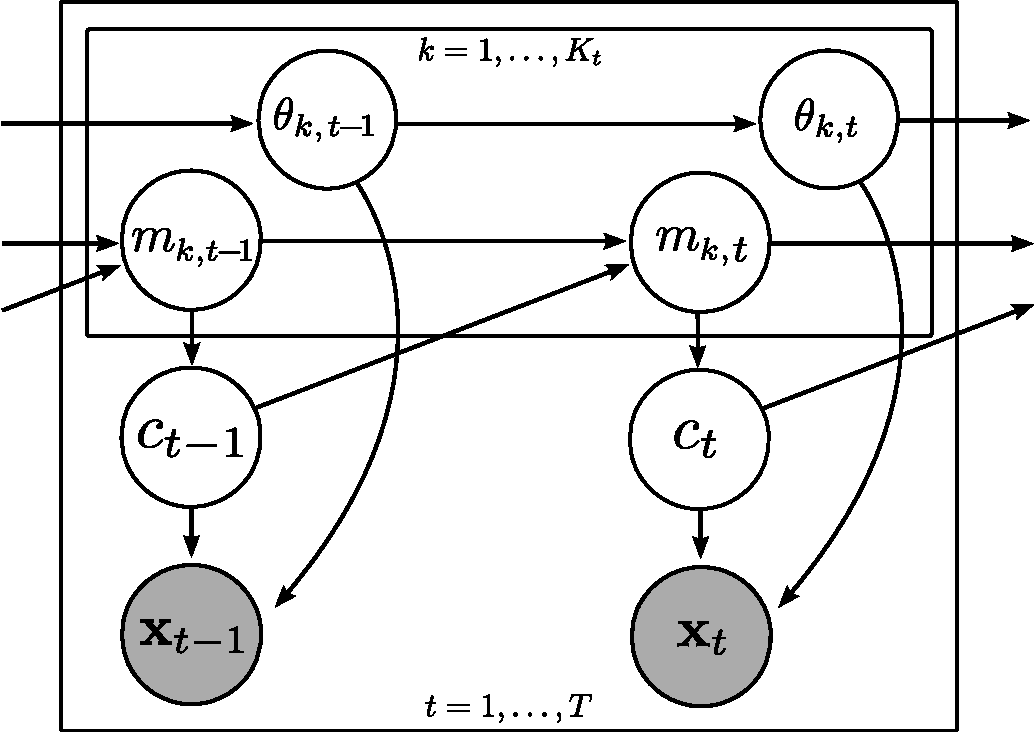
\includegraphics[width=80mm]{../img/gpuddp_gm_1.pdf}}
        \caption{\label{fig:gpuddpm_gm_1} Graphical Model of the Generalized Polya Urn Dependent Dirichlet Process Mixture. Note that all observations at time $t$, $\bold{x}_{1:N,t}$, and their associated assignments $c_{1:N,t}$ are denoted respectively as $\bold{x}_{t}$ and $c_{t}$ (this also holds for time step $t-1$).}
\end{figure}


\subsection{Deletion Variable Formulation of the GPUDDPM}

To allow for modeling time-dependent data, the GPUDDPM allows clusters to ``lose'' assigned observations in a deletion step, which modifies the values of the cluster sizes at each time. Instead of incorporating the cluster size variable $m$ directly in the model (as it was in the definition of the GPUDDPM given by \eqref{gpuddpm_def}), we can formulate an equivalent model which makes use of new set of variables called the deletion variables (denoted as $d$), which represent the times at which assignments are deleted. More precisely, we introduce variables $d_{1}, \ldots, d_{N}$ to the model, which denote the times at which the assignments of observations $1, \ldots, N$ are considered removed from their assigned cluster. At each time step, cluster sizes can be recontructed from all previous assignment and deletion variables. With these deletion variables, we can compute the size of cluster $k$ at time $t$, $m_{k,t}$, by
\begin{equation}
\label{compute_clust_size}
m_{k,t} = \sum_{t' = 1}^{t} \mathbb{I}[(c_{t'}=k) \wedge (t < d_{t'})]
\end{equation}
where $\mathbb{I}[\cdot]$ is an indicator function that evaluates to 1 if its argument is true, and 0 otherwise. Additionally, for an observation $\bold{x}_{i}$ at a given time-step $t$, the deletion time $d_{i}$ can be defined to be $d_{i} = t + l_{i}$, where $l_{i}$ is considered the lifespan of an assignment, is distributed geometrically, and can be expressed as
\begin{equation}
\label{del_rho_form}
l_{i} | \rho  \sim  \rho(1 - \rho)^{l_{i}}
\end{equation}
This alternate, deletion variable formulation of the GPUDDPM is useful for the MCMC inference algorithm described in Section~\ref{sec:MCMC}. We can write the new formulation of the GPUDDPM as, for each time step $t \in \{1, \ldots, T\}$ and clusters $k \in \{ 1, \ldots, K_{t} \} $ at time $t$,
\begin{align}
\begin{split}
d_{i,t} | \rho  &\sim \text{Geo}(\rho) + t + 1 \\
\theta_{k, t} | \theta_{k, t-1}  &\sim
\begin{cases}
P(\theta_{k,t} | \theta_{k,t-1}) \hspace{2mm} \text{if} \hspace{2mm} k \in \{ 1, \ldots, K_{t} \} \\
\mathbb{G}_{0} \hspace{2mm} \text{if} \hspace{2mm} k = K_{t} + 1
\end{cases} \\
c_{i,t} | \bold{c}_{1:t-1}, \bold{d}_{1:t-1}, \alpha  &\sim  \text{C}(\bold{c}_{1:t-1}, \bold{d}_{1:t-1}, \alpha) \\
\bold{x}_{i,t} | c_{i,t}, \theta_{c_{i,t},t}  &\sim  \text{F}(\theta_{c_{i,t}, t})
\end{split}
\end{align}
where $\bold{c}_{t} = c_{1,t}, \ldots, c_{N_{t}, t}$ (for $N_{t}$ observations at time $t$), $\bold{d}_{t} = d_{1,t}, \ldots, d_{N_{t}, t}$, and we specify distributions for F, $\mathbb{G}_{0}$, and $P(\theta_{k, t} | \theta_{k, t-1})$ in Section~\ref{sec:modelspecification}. This formulation of the GPUDDPM is also used by \cite{gasthaus_thesis} and \cite{caron_2007}. The associated graphical model for this formulation is given in Figure~\ref{fig:gpuddpm_gm_2}.
\begin{figure}[h]
        \center{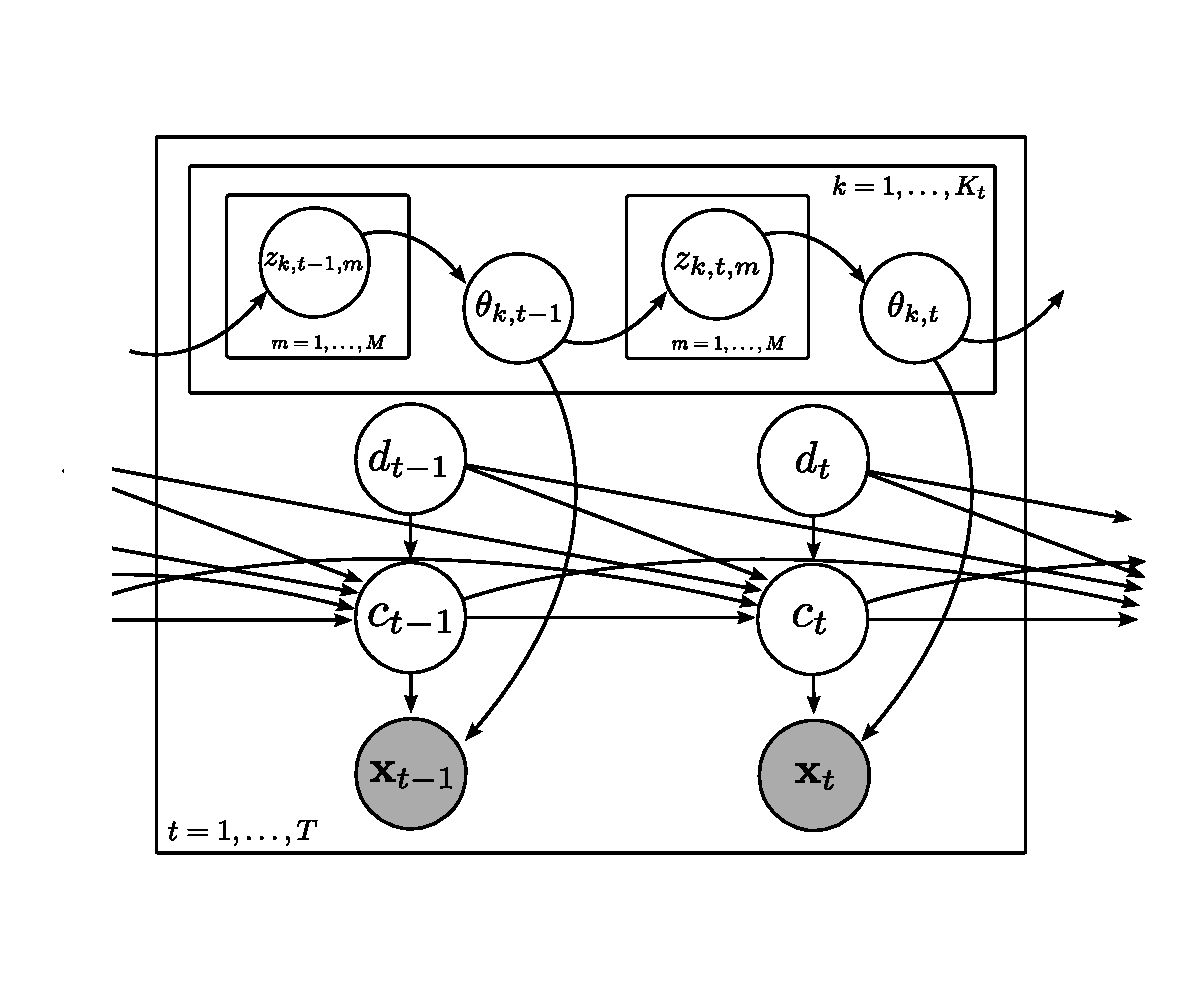
\includegraphics[width=82mm]{../img/gpuddp_gm_3.pdf}}
        \caption{Graphical model of the deletion variable and auxiliary variable transition kernel representation of the GPUDDPM}
        \label{fig:gpuddpm_gm_2}
\end{figure}



% Model Specification
% -------------------

\section{Model Specification}
\label{sec:modelspecification}

Sections~\ref{sec:objectappearance}-\ref{sec:motionmodel} describe the distributions chosen to fully specify the general GPUDDPM model form given in Section~\ref{sec:modeloverview}. The implementation given below was used for all the experiments of Section~\ref{sec:experiments}.


\subsection{Object Appearance (Mixture Component)}
\label{sec:objectappearance}

At a given time $t$, we model each observation $\bold{x} \in \bold{X}$ as a draw from the product of a multivariate normal and multinomial distribution
\begin{equation}
\label{likelihood}
\text{F}(\bold{x}|\theta) = \mathcal{N}(\bold{x}^{s} | \boldsymbol{\mu}, \Sigma)  \mathcal{M}n(\bold{x}^{c} | \bold{p})
\end{equation}
where $\theta = \{ \boldsymbol{\mu}, \Sigma, \bold{p} \}$ denote the parameters of a cluster at time $t$, with mean $\boldsymbol{\mu} \in \mathbb{R}^{2}$, covariance matrix $\Sigma \in \mathbb{R}^{2} \times \mathbb{R}^{2}$, and discrete probability vector $\bold{p} = (p_{1}, \ldots, p_{V})$ such that $\sum_{i=1}^{V}p_{i} = 1$. Additionally, $\mathcal{N}$ denotes the multivariate normal distribution, $\mathcal{M}n$ denotes the multinomial distribution, and F is sometimes referred to as the likelihood.

The distribution families assumed to generate each $\bold{x}$ must be justified. Both the multivariate normal and multinomial distributions were chosen because they are sufficiently simple (and well studied) to allow for tractable inference and sufficiently flexible to provide a reasonable approximation to the data gained during extraction. In particular, the multivariate normal distribution over the spatial features $\bold{x}^{s}$ can be thought to represent the shape of each object as an oval; likewise, data generated by each moving object during extraction are often ovular---as noisy extraction procedures cause some smoothing of edges and corners, producing blob-like shapes even when objects are not particularly round---and centered on a given object.
Furthermore, this model is justified as the maximum likelihood parameter estimate of a normal distribution corresponds to the least squares fit of data relative to the normal distribution mean; since extraction data produced by an object clusters around the centroid of the object, the estimated normal distribution mean should provide a reasonable reflection of the object's centroid.
Modeling the color features $\bold{x}^{c}$ as draws from a multinomial distribution (equivalently, as draws from a product of discrete distributions), is justified since we have observed that distinct object tend to generate pixels whose hue values are noisy but yield consistent counts in discrete hue bins.


\subsection{Appearance Prior (Base Distribution)}
\label{sec:appearanceprior}

$\mathbb{G}_{0}$ denotes the base distribution of the time-dependent Dirichlet process mixture; it also serves as a prior distribution for the parameters $\theta = \{ \boldsymbol{\mu}, \Sigma, \bold{p} \}$ present in the mixture components (i.e. the parameters we've used to model object appearance). We make use of conjugate priors in the base distribution to allow for more efficient computation. Specifically, in the experiments carried out in this paper, a normal-inverse-Wishart prior is placed on the multivariate normal parameters $\{ \boldsymbol{\mu}, \Sigma \}$, and a Dirichlet prior is placed on the multinomial parameter $\bold{p}$ (where the normal-inverse-Wishart is a conjugate prior for the multivariate normal component of the likelihood and the Dirichlet is a conjugate prior for the multinomial component). The prior can therefore be written
\begin{equation}
\label{basedistro}
\mathbb{G}_{0}(\theta) = \mathcal{N}i\mathcal{W}(\boldsymbol{\mu}, \Sigma | \boldsymbol{\mu}_{0}, \kappa_{0}, \nu_{0}, \Lambda_{0})  \mathcal{D}ir( \bold{p} | \bold{q}_{0})
\end{equation}
where $\mathcal{N}i\mathcal{W}$ denotes the normal-inverse-Wishart distribution, $\mathcal{D}ir$ denotes the Dirichlet distribution, and the prior has the hyperparameters $\boldsymbol{\mu}_{0}, \kappa_{0}, \nu_{0}, \Lambda_{0}$ and $\bold{q}_{0}$.


\subsection{Motion Model (Transition Kernel)}
\label{sec:motionmodel}

We wish to formulate a transition kernel $P(\theta_{t} | \theta_{t-1})$ that provides a reasonable representation of how we expect tracked objects to move over time. In the interest of formulating a model with the intention of using it to track arbitrary objects, we do not wish to make many assumptions about the long-term behavior of objects. For example, we choose not to adopt a transition kernel that incorporates object dynamics, though a transition kernel that models this or other sophisticated behavioral tendencies could potentially be implemented in future works if one knows that they are consistent characteristics of an object's movement.

As described in Section~\ref{sec:gpuddpm}, $\mathbb{G}_{0}$ must be the invariant distribution of $P(\theta_{t} | \theta_{t-1})$ in order for the the cluster parameters to remain marginally distributed according to the base distribution. In other words, the transition kernel must satisfy
\begin{equation}
\int \mathbb{G}_{0}(\theta_{t-1})P(\theta_{t} | \theta_{t-1}) d\theta_{t-1} = \mathbb{G}_{0}(\theta_{t})
\end{equation}
for a given cluster with parameters $\theta$. One way to achieve this is through the use of auxiliary variables. Auxiliary variables are a set of $M$ variables $\bold{z}_{t} = (z_{t,1}, \ldots, z_{t,M})$ associated with a each cluster at time $t$ that satisfy
\begin{eqnarray}
% P(\theta_{k,t} | \theta_{k,t-1}) = \int P(\theta_{k,t} | \bold{z}_{k,t}) P(\bold{z}_{k,t} | \theta_{k,t-1}) d \bold{z}_{k,t}
P(\theta_{t} | \theta_{t-1}) = \int P(\theta_{t} | \bold{z}_{t}) P(\bold{z}_{t} | \theta_{t-1}) d \bold{z}_{t}  %\\
% P(\theta', \bold{z}_{t}) = p(\bold{z}_{t}|\theta') \mathbb{G}_{0}(\theta')
\end{eqnarray}

In this way, the parameters of a cluster at a given time do not depend directly on their value at the previous time; they are instead dependent upon an intermediate sequence of auxiliary variables chosen to satisfy the above criteria, which allows the cluster parameters at each time step to be marginally distributed according to the base distribution $\mathbb{G}_{0}$.

For each cluster, we introduce $M$ auxiliary variables $z_{t, 1}, \ldots, z_{t, M}$ at time $t$ that are each drawn from the product of a multivariate normal and multinomial when conditioned on the associated cluster parameters $\theta_{t} = \{ \boldsymbol{\mu}_{t}, \Sigma_{t}, \bold{p}_{t} \}$:
\begin{equation}
\label{transker1}
z_{t, m} | \boldsymbol{\mu}_{t}, \Sigma_{t}, \bold{p}_{t}  \sim  \mathcal{N}(\boldsymbol{\mu}_{t}, \Sigma_{t}) \mathcal{M}n(\bold{p}_{t})   \hspace{15pt}   
\forall m \in \{ 1, \ldots, M \}
\end{equation}
To satisfy the above criteria for auxiliary variables, at each time $t$ we specify the dependencies of a given cluster on its associated set of auxiliary variables by
\begin{equation}
\label{transker2}
\boldsymbol{\mu}_{t}, \Sigma_{t}, \bold{p}_{t} | \bold{z}_t  \sim  \mathcal{N}i\mathcal{W}(\boldsymbol{\mu}_{M}, \kappa_{M}, \nu_{M}, \Lambda_{M})  \mathcal{D}ir(\bold{q}_{M})
\end{equation}
where $\boldsymbol{\mu}_{M}, \kappa_{M}, \nu_{M}, \Lambda_{M},$ and $\bold{q}_{M}$ are parameters given by
\begin{eqnarray}
\kappa_{M} &=& \kappa_{0} + M \\
\nu_{M} &=& \nu_{0} + M \\
\boldsymbol{\mu}_{M} &=& \frac{\kappa_{0}}{\kappa_{0}+M} \boldsymbol{\mu}_{0}  +  \frac{M}{\kappa_{0}+M} \overline{\bold{z}_t}^{s}\\
\Lambda_{M} &=& \Lambda_{0} + S_{\bold{z}_{t}^{s}}\\
\bold{q}_{M} &=& \bold{q}_{0} + \sum_{m=1}^{M} z_{t,m}^{c}
\end{eqnarray}
where $M$ is the number of auxiliary variables, \\
$\{ \boldsymbol{\mu}_{0}, \kappa_{0}, \nu_{0}, \Lambda_{0} \}$ are the $\mathcal{N}i\mathcal{W}$ prior parameters, $\bold{q}_{0}$ is the $\mathcal{D}ir$ prior parameter, $\bold{z}^{s}$ and $\bold{z}^{c}$ respectively denote the spatial and color features of an auxiliary variable $\bold{z}$, and $\overline{\bold{z}}$ and $S_{\bold{z}}$ respectively denote the sample mean and sample covariance for a set $\bold{z} = \{ z_{1}, \ldots, z_{M} \}$ (of auxiliary variables, in this case), which we can define as
\begin{eqnarray}
\label{samplemean}
\overline{\bold{z}}  &=&  \left( \sum_{m=1}^{M} z_{m} \right) / M\\
\label{samplecov}
S_{\bold{z}}  &=&  \sum_{m=1}^{M} (z_{m} - \overline{\bold{z}}) (z_{m} - \overline{\bold{z}})^{T}
\end{eqnarray}


\subsection{Recap of Parameters in Model}
\label{sec:recapofparameters}

The multivariate normal-multinomial GPUDDPM implemented in this study has a number of parameters, which can be tuned to increase the efficacy of object detection and tracking. \\ \\
Object appearance parameters include:
\begin{center}
\begin{tabular}[c]{l p{7cm}}
$\boldsymbol{\mu}_{0}$  &  The mean prior. In experiments performed in Section~\ref{sec:experiments} the data was recentered to the origin, and this parameter was set to $(0,0)$ \\
$\kappa_{0}$  &  scale factor of the variance of the prior on the mean\\
$\nu_{0}$  &  scale factor of the variance of the prior on the covariance\\
$\Lambda_{0}$  &  shape factor of the prior on the covariance\\
$\bold{q}_{0}$  &  scale factor of the prior on the multinomial counts
\end{tabular}
\end{center} \vspace{3mm}
The following parameter dictates characteristics involving the movement of objects
\begin{center}
\begin{tabular}[c]{l p{7cm}}
$M$  &  Number of auxiliary variables. A large number will produce lower variation in position (better for slower objects) and a low number will produce higher variation in position.
\end{tabular}
\end{center} \vspace{3mm}
Additionally, one can tune the model's tendency to detect new objects and maintain the existence of these objects (or the rate at which objects become inactive or leave the video) with the following parameters
\begin{center}
\begin{tabular}[c]{l p{7cm}}
$\alpha$  &  The granularity parameter for the Dirichlet Process. A higher value will increase the tendency for new objects to be detected.\\
$\rho$  &  The deletion parameter. A higher value will give objects an increased tendency to die off.
\end{tabular}
\end{center}

We have not found an easily justifiable way to choose parameters. For the appearance and movement parameters, samples were drawn given a range of parameter values, and those that yielded samples similar in appearance to the experimental data were kept (a technique also performed in \cite{gasthaus_thesis}). The parameters chosen for use in experiments (Section~\ref{sec:experiments}) were accepted based on the fact that they yielded reasonable results. Additionally, a sensitivity analysis was carried out for the granularity and deletion parameters ($\alpha$ and $\rho$), where a range of values for both were chosen, and inference performed for each; results of this analysis are discussion in Section~\ref{sec:sensitivityanalysis}.



% Inference
% ---------

\section{Inference}
\label{sec:inference}


\subsection{MCMC: Batch Inference}
\label{sec:MCMC}


\subsection{SMC: Sequential Inference}
\label{sec:SMC}


\subsection{From Inference to Tracking Results}
\label{sec:inferencetotrackingresults}

% The multivariate normal-multinomial model on which inference is described in this section can be used to gain object detection and tracking results. The nature of object detection and tracking results may vary depending on the application or performance metrics used (see Section~\ref{sec:performance_metrics}); in this study, we desire the centroid position and approximate spatial region for each moving object, for each frame that this object can be seen within the video. We choose to make our detection and tracking results depend completely on the inferred parameters of the multivariate normal distribution of each cluster. Each inferred cluster was taken to be a distinct detected object, and the sequence of means and covariance matrices for a given cluster were used, respectively, to determine the position and spatial region of a given object over a sequence of time steps. In particular, the mean parameter was taken to be the centroid of an object, and a 2-dimensional oval denoting a boundary around the mean that contains a specified percentage of the data (where the specification for this oval is given in Section~\ref{sec:pets2000_2001}) was taken to be the spatial region of the object. Furthermore, as both provided inference methods use sampling, and each sample represents a result, we must choose a way to narrow these down to a single result. We have found that calculating the joint log probability for each sample and choosing the sample that yields the highest value as a result works reasonably well.



% Experiments
% -----------

\section{Experiments}
\label{sec:experiments}


\subsection{Performance Evaluation Metrics}
\label{sec:performanceevaluationmetrics}


\subsection{Synthetic Video Datasets}
\label{sec:syntheticvideodatasets}


\subsection{Benchmark Video Datasets}
\label{sec:benchmarkvideodatasets}


\subsubsection{PETS2000 and PETS2001}
\label{sec:pets2000and2001}

\subsubsection{PETS2009/2010}
\label{sec:pets20092010}

\subsubsection{Sensitivity Analysis}
\label{sec:sensitivityanalysis}



% Conclusion
% ----------

\section{Conclusion}
\label{sec:conclusion}



\begin{small}
\bibliographystyle{plainnat}
\bibliography{paper_refs} 
\end{small}



\end{document}